\documentclass[tikz,border=6pt]{standalone}
\usepackage[T1]{fontenc}
\usepackage{lmodern}
\usepackage{amsmath,amssymb}
\usetikzlibrary{positioning,arrows.meta,fit,calc}
% Design of koblitz-n83-rankprobe-20261019 (frozen protocol.json). Not a result.
\begin{document}
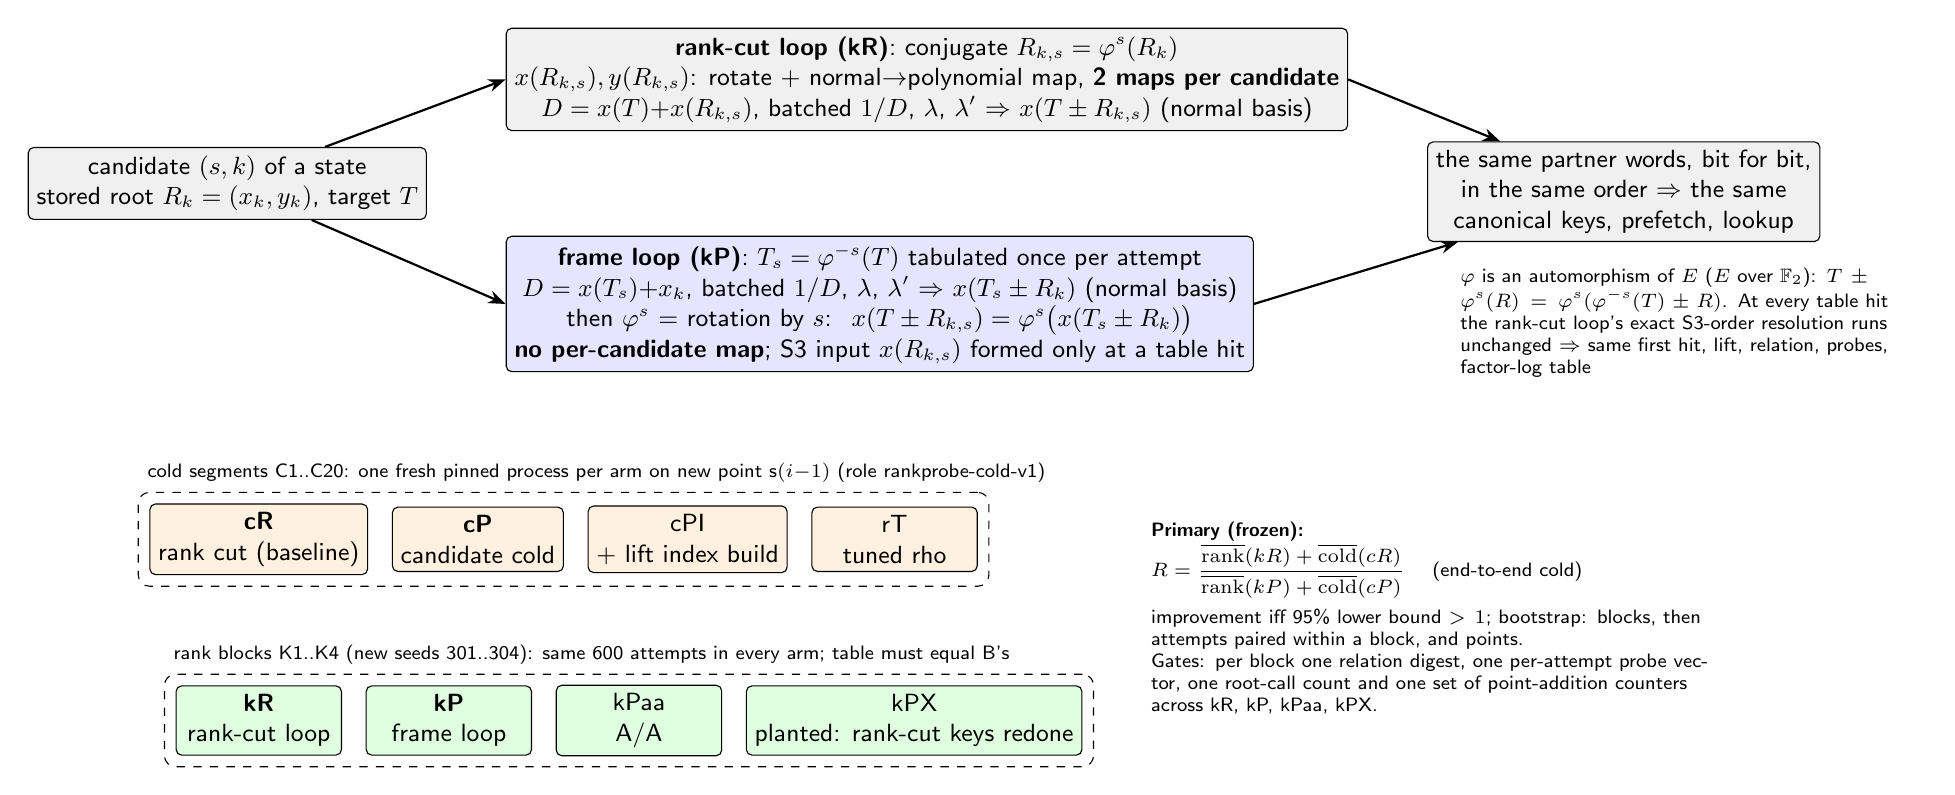
\begin{tikzpicture}[
  font=\sffamily\small,
  box/.style={draw, rounded corners=2pt, align=center, minimum height=8mm, inner sep=3pt},
  base/.style={box, fill=gray!12},
  add/.style={box, fill=blue!10},
  arm/.style={box, fill=orange!12, minimum width=21mm},
  rank/.style={box, fill=green!12, minimum width=21mm},
  arr/.style={-{Stealth[length=2.2mm]}, thick},
  note/.style={align=left, font=\sffamily\scriptsize}
]
% One candidate of one state: stored root R_k, Frobenius shift s, rank target T
\node[base] (in) {candidate $(s, k)$ of a state\\stored root $R_k=(x_k, y_k)$, target $T$};
\node[base, above right=2mm and 10mm of in] (rc) {\textbf{rank-cut loop (kR)}: conjugate $R_{k,s}=\varphi^s(R_k)$\\
$x(R_{k,s}), y(R_{k,s})$: rotate + normal$\to$polynomial map, \textbf{2 maps per candidate}\\
$D=x(T){+}x(R_{k,s})$, batched $1/D$, $\lambda$, $\lambda'$ $\Rightarrow$ $x(T\pm R_{k,s})$ (normal basis)};
\node[add, below right=2mm and 10mm of in] (fr) {\textbf{frame loop (kP)}: $T_s=\varphi^{-s}(T)$ tabulated once per attempt\\
$D=x(T_s){+}x_k$, batched $1/D$, $\lambda$, $\lambda'$ $\Rightarrow$ $x(T_s\pm R_k)$ (normal basis)\\
then $\varphi^s$ = rotation by $s$: \ $x(T\pm R_{k,s})=\varphi^s\big(x(T_s\pm R_k)\big)$\\
\textbf{no per-candidate map}; S3 input $x(R_{k,s})$ formed only at a table hit};
\draw[arr] (in) -- (rc.west); \draw[arr] (in) -- (fr.west);
\node[base, anchor=west] (keys) at ($(fr.east)!0.5!(rc.east) + (16mm,0)$) {the same partner words, bit for bit,\\in the same order $\Rightarrow$ the same\\canonical keys, prefetch, lookup};
\draw[arr] (rc.east) -- (keys); \draw[arr] (fr.east) -- (keys);
\node[note, anchor=north west, text width=58mm] (ex) at ($(keys.south west)+(3mm,-2mm)$) {$\varphi$ is an automorphism of $E$ ($E$ over $\mathbb{F}_2$): $T\pm\varphi^s(R)=\varphi^s(\varphi^{-s}(T)\pm R)$.
At every table hit the rank-cut loop's exact S3-order resolution runs unchanged $\Rightarrow$ same first hit, lift, relation, probes, factor-log table};

% Cold arms
\node[arm, below=36mm of in, xshift=4mm] (cR) {\textbf{cR}\\rank cut (baseline)};
\node[arm, right=3mm of cR] (cP) {\textbf{cP}\\candidate cold};
\node[arm, right=3mm of cP] (cPI) {cPI\\+ lift index build};
\node[arm, right=3mm of cPI] (rT) {rT\\tuned rho};
\node[draw, dashed, rounded corners, fit=(cR) (rT), inner sep=4pt, label={[note, anchor=south west]north west:{cold segments C1..C20: one fresh pinned process per arm on new point s$(i{-}1)$ (role rankprobe-cold-v1)}}] (cold) {};

% Rank arms
\node[rank, below=14mm of cR] (kR) {\textbf{kR}\\rank-cut loop};
\node[rank, right=3mm of kR] (kP) {\textbf{kP}\\frame loop};
\node[rank, right=3mm of kP] (kPaa) {kPaa\\A/A};
\node[rank, right=3mm of kPaa] (kPX) {kPX\\planted: rank-cut keys redone};
\node[draw, dashed, rounded corners, fit=(kR) (kPX), inner sep=4pt, label={[note, anchor=south west]north west:{rank blocks K1..K4 (new seeds 301..304): same 600 attempts in every arm; table must equal B's}}] (rk) {};

\node[note, anchor=west, text width=72mm] (eq) at ($(rk.east)+(6mm,13mm)$) {\textbf{Primary (frozen):}\\
$R = \dfrac{\overline{\mathrm{rank}}(kR) + \overline{\mathrm{cold}}(cR)}{\overline{\mathrm{rank}}(kP) + \overline{\mathrm{cold}}(cP)}$ \quad (end-to-end cold)\\[1mm]
improvement iff 95\% lower bound $>1$; bootstrap: blocks, then attempts paired within a block, and points.\\
Gates: per block one relation digest, one per-attempt probe vector, one root-call count and one set of point-addition counters across kR, kP, kPaa, kPX.};
\end{tikzpicture}
\end{document}
